\documentclass[15pt]{report}
%\usepackage[utf8]{inputenc}
\usepackage{graphicx}
\usepackage{fancyhdr}
\pagestyle{fancy}
\usepackage{amssymb}
\usepackage{bbm}
\graphicspath{ {images/} }
\usepackage[backend=bibtex]{biblatex}
\usepackage{graphicx}

\usepackage{listings}
\usepackage{color}

\definecolor{dkgreen}{rgb}{0,0.6,0}
\definecolor{gray}{rgb}{0.5,0.5,0.5}
\definecolor{mauve}{rgb}{0.58,0,0.82}

\lstset{frame=tb,
  language=Python,
  aboveskip=3mm,
  belowskip=3mm,
  showstringspaces=false,
  columns=flexible,
  basicstyle={\small\ttfamily},
  numbers=none,
  numberstyle=\tiny\color{gray},
  keywordstyle=\color{blue},
  commentstyle=\color{dkgreen},
  stringstyle=\color{mauve},
  breaklines=true,
  breakatwhitespace=true,
  tabsize=3
}
\lstnewenvironment{code}%
  {\noindent\minipage{\linewidth}
   \lstset{}}
  {\endminipage}


\renewcommand*{\arraystretch}{1.5}

\newcommand{\dx}[1]{ \frac{\partial}{\partial x^{#1} }}
\newcommand{\dxx}[2]{ \frac{\partial x^{#1}}{\partial x^{#2} }}

\bibliography{ref1}
\setcounter{tocdepth}{3}
\title{PyGravity \\
		\small http://github.com/russloewe/PyGravity}

\author{Russell Loewe}

\date{7~May 2015}

\begin{document}

\maketitle

\indent
This is the supporting documentation for
\textit{PyGravity} 

\tableofcontents
% \setcounter{section}{-1}

\newpage



\section{Intro}
\indent \paragraph{Purpose} This is a gravity simulator written in Python and using PyGame as a render. This project is starting at the basics of using vector calculus and Newtons law of Gravity to calculate the paths of particles with respect to the gravity exerted by neighbouring particles. One of many end goals with this simulator is to simulate asteroids colliding into more massive asteroids, eventually becoming planets.
\indent \paragraph{Context} This simulator is going to be dealing with non-relativistic energies in flat space-time. That means every object can be given by a Euclidean 3-space vector. Instead of dealing with the 4 coordinates of space-time, I will assume that every object shares the same clock and thus time will be kept globally by the physics engine. 
\indent \paragraph{Vectors}I am writing my own library for  the various mathematical operations that will be need to calculate the forces. The library is going to start off with the basic vector objects. I will then add functions on vector objects such as addition, subtraction, multiplication by a scalar, normalizing, finding orthogonal vectors, and etcetera. At this point and for the rest of the application I will use Numpy to handle the large or small numbers that are going to be needed in calculations.
\indent \paragraph{Objects} I am also going to need to create a class object to encapsulate the particles. This class will contain the needed attributes of each particle such as the scalar mass, the vectors of position and velocity.The classes will also need to contain procedures for particle collisions. This will most likely not be need until later when I use this simulate to for colliding asteroids.
\indent \paragraph{Physics} After the math foundation and base object classes are established then I will need to develop a physics library to calculate physics specfic formulaes such as the force of gravity, acceleration and the net force of gravity for more than two objects.
\indent \paragraph{PyGame} Once I have a foundation of vector math built into my simulator I will then move on to using PyGame to plot the position of various particles and then render their movement. PyGame will be used to render the evolution of the dynamical system and also display various stats of the particles. I will also pause at this point to use PyGame to graph the gradient of gravity in the system and other fun stuff.

%\section{Physics and Math Refresher}


\chapter{Basic Math and Physics}

\section{The Vector Class} \label{vectors}
\subsection{Vector Base} First thing is to have a code representation of a vector. A vector in 3-space needs to have three components. The general vector class is structured as follows:

\begin{code}

class Vector(object):
    def __init__(self, x, y, z):
        self.x = x
        self.y = y
        self.z = z
        self.show = "(" + str(self.x) + ',' + str(self.y) + ',' + str(self.z) + ')'
           

\end{code}

The vector is initialized with the three components. The \textit{\_\_init\_\_} method also contains the attribute \textit{show}, which is an easy way to view the vector in string format for interactive sessions. Thus a new vector, $\vec{A}$, is created and displayed by

\begin{code}
A = Vector(1.1, 1.3, 1.4)
A.show
'(1.1, 1.3, 1.4)'
\end{code}

\subsection{Addition} Next method to add to the base vector class is the function for adding two vectors. Vector addition is going to be a static class method of the Vector Class which takes two vectors and returns a new vector.

\begin{code} 
    @staticmethod
    def add(A, B):
        new = Vector(A.x + B.x, 
                     A.y + B.y,
                     A.z + B.z)
        return new
\end{code}

Thus to find $\vec{C} =\vec{A} + \vec{B}$, we would use this

\begin{code}
A = Vector(1,1,1)
B = Vector(2,1,3)
C = Vector.add(A,B)
C.show
'(3,2,4)'
\end{code} 

The test suite ensures that this addition holds true for positive and negative integers, and real numbers up to $10^{24}$. It is important to note that boolean operations are only guaranteed to hold true when comparing two vector components, not necessarily a vector component and an isolated number. Example below.

\begin{code}
BigA = Vector(1.3*10**24, 0, 0)
BigB = Vector(1.1*10**24, 0, 0)
Answer = Vector(2.4*10**24, 0, 0)
C = Vector.add(BigA, BigB)

C.x == Answer.x        ::True
C.x == 2.4*10**24      ::False
\end{code} 

\subsection{Subtraction}Subtraction is coded exactly like addition except that each component of $\vec{A}$ is subtracted by each cmponent of $\vec{B}$. The first function argument is the minuend and the second argument is the subtrahend. Example:

\begin{code}
A = Vector(1,1,1)
B = Vector(2,2,2)
Vector.sub(A, B) = (-1, -1, -1)
Vector.sub(B, A) = (1, 1, 1)
\end{code}

\subsection{Scalar Multiplication} Next the Vector Class needs a method for multiplying vectors by a scalar. The multiplication method will be very similar to the addition method.

\begin{code}
@staticmethod
def times_scalar(a, A):
    new = Vector(A.x * a, 
                 A.y * a,
                 A.z * a)
    return new
\end{code}

This method returns a new vector, thus usage is as following:

\begin{code}
A = Vector(1.1, 2.2, 4.4)
a = 2.0
C = Vector.times_scalar(a, A)
C.show
'(2.2, 4.4, 8.8)'
\end{code}

For testing there were problems when working with large numbers. The computation could be correct but the answer wouldn't pass the tests because of small errors resulting from working with such large numbers. Thus rounding would be needed so only significant figures would be compared. Here is a quick rounding to significant digits function taken from \textit{StackOverflow}\cite{indgar} along with a tweak to avoid math domain errors.

\begin{code}
from math import log10, floor
def round_sig(x, sig=2):
    if x == 0:
        return 0
    if x < 0:
        x = -x
        return (-1)* round(x, sig-int(floor(log10(x)))-1)
    else:
        return round(x, sig-int(floor(log10(x)))-1)

\end{code}

Then the tests look like this:

\begin{code}
self.failUnless(C.x == Ans.x )            
self.failUnless(round_sig(C.y, 2) == round_sig(Ans.y, 2))
\end{code}

The first line above won't hold true for large numbers with more than two significant digits. The second line will hold true since it cuts off the computer error, but preservers the significant digits.
\subsection{Magnitude} The next function needed is finding the magnitude of a vector. The equation for the magnitude of an \textit{Euclidean} 3-space vector is 
\begin{equation}
\left| \vec{V} \right|  = \sqrt{dx^2 + dy^2 + dz^2}
\end{equation}
The code is still pretty straight forward:

\begin{code}
@staticmethod
def magnitude(A):
   mag = math.sqrt(A.x**2 + A.y**2 + A.z**2)
   return mag
\end{code}

And usage is straight forward too

\begin{code}
A = Vector(5, 8, 10)
B = Vector(3, 1, 2)
Vector.magnitude(A)                     # = 13.7
Vector.magnitude(B)                     # = 3.7
Vector.magnitude(Vector.sub(A,B))       # = 10.8
\end{code}

The last line gives us the distance between $\vec{A}$ and $\vec{B}$.

\section{The Particle Class}
The particle class is the object that will encapsulate the velocity, positional vectors and mass scalar of various point particles. To come will be an attribute for the radius of the particle for collisions and growth but for now we will be working with point particles.

\subsection{Particle Base} The base class for the particle needs to include a information for where the particle is, how fast it is moving and how heavy it is. Therefore the Particle Class needs three attributes: two vectors and one scalar.

\begin{code}
from Vector import Vector

class Particle(object):
    def __init__(self, P, V, m):
        self.P = P        #particle's position vector
        self.V = V        #Particle's velocity vector
        self.m = m        #particle's mass
\end{code}

\subsection{Movement} The particle needs to be moved. For each tick of time, $\Delta t$, the particle is displaced by its velocity vector. Thus at time $t$, the particle $a$ has a positional vector $\vec{P}_{a}(t)$ and velocity vector $\vec{V}_{a}(t)$. Thus if the position and velocity are know at $t=n$, then the position at $t = n+1$ can be given by

\begin{equation}
 \vec{P}_a (t_{n+1}) = \vec{P}_{a}(t_n) + \vec{V}_a (t_n)
\end{equation}

Utilizing the previous vector addition function the above equation is easily given by the method function:

\begin{code}
def move(self):
    new_pos = Vector.add(self.P, self.V)
    self.P = new_pos
\end{code}

The usage is really simple. When it comes time to move the particle we simply call move(): 

\begin{code}
a = Particle(Vector(1,1,1), Vector(1,2,-3)
a.move()
print a.P.show		#display pos vector
'(2, 3, -2)'   
\end{code}

The new position is then calculated using the current position and velocity of the vector.

\subsection{Acceleration} The particle is going to be moving in gravitational fields and therefore must be able to be accelerated. At some particular time $t$ there will be a gravitational force acting on the particle. This force will be a force vector $\vec{F}$. The acceleration will then be found by $\vec{a} = \frac{\vec{F}}{m}$, where $m$ is the mass of the particle in question. The acceleration will not need to be saved as an attribute of the particle because it is calculated for each $t_n$ and does not depend on the acceleration at $t_{n-1}$. What does need to happen is at each time interval, after the acceleration is calculated, the acceleration vector will be added to the particle's velocity vector. Therefore the velocity of particle $A$ at $t = {n + 1}$ is given by 
\begin{equation}
\vec{V}_a (t_{n+1}) = \vec{V}_a (t_n) + \vec{A}_a (t_n)
\end{equation}

The particle's method function to apply acceleration closely resembles the function to move the particle, however it takes the acceleration as an argument since acceleration is not stored with the particle.  The function is given by

\begin{code}
def accelerate(self, A):
    new = Vector.add(self.V, A)
    self.V = new
\end{code}

Usage first requires that the acceleration acting on the particle is calculated. This will come in the next chapter when the physics calculations are formed. For now I will use explicitly define the acceleration vector.

\begin{code}
Vol_vec = Vector(1, 1, 1)
Acc_vec = Vector(2, 2, -1)
p = Particle(Pos_Vec, Vol_vec, mass)
p.accelerate(Acc_vec)
print p.V.show		#display vol vector
'(3, 3, 0)'
\end{code}

\section{Physics}
This section of code is going to contain the Physics class. This class will have a list attribute for keeping track of all the particles and class methods for calculating the force of gravity in the system. The Physics class will depend on the Vector and Particle classes but will be separated for easier editing down the road.
\subsection{Physics Base} The base class takes no arguments. It has a list as an attribute that holds the various particles in the system. Right away I'm going to add the method for adding particles to the attribute list. The implementation also depends on the Particle class.

\begin{code}
from Vector import Vector
from Particle import Particle
class Physics(object):
    def __init__(self):
        self.objects = []
        
    def add_obj(self, obj):
        self.objects.append(obj)
\end{code}
 
To use first create a Physics Class object then particles can be add using the Physics Class method. 

\begin{code}
from libs import Vector, Particle, Physics

system = Physics()
part1 = Particle(Vector(1,1,1), (1,1,1), 5)
part2 = Particle(Vetor(5,.3,2), Vector(.2, 0, .1), 100)

system.add_obj(part1)
system.add_obj(part2)

\end{code}

\subsection{Force of Gravity}
Now we are ready to start calculating the force of gravity between two particles. This section is going to use the familiar Newtonian force of gravity,
\begin{equation} \label{grav}
F = \frac{G m_1 m_2}{R^2} 
\end{equation}
where, \\
$G$ = Gravitational constant \\
$m_1$ = mass of particle 1 \\
$m_2$ = mass of particle 2 \\
$r$ = distance between particle 1 and 2

\paragraph{} The above equation only gives the magnitude of the force of gravity. The for the simulation the vector form is need. We already have the magnitude, now all we need is direction which is given by the unit vector pointing from particle 1 to particle 2. 
\paragraph{} Instead of $r$ in the above equation let's instead take $\vec{R}$ and define it as the displacement vector :
\begin{equation}\label{r_displace}
\vec{R} = \vec{P_2} - \vec{P_1}
\end{equation}
where $P_1$ and $P_2$ are the position vectors for both respective particles in question. Then the magnitude of $\vec{R}$ is noted as $\| \vec{R} \| $. Thus the unit vector pointing in the direction of $\vec{R}$ is $\hat{R} = \frac{\vec{R}}{\| \vec{R} \|}$. Now we can rewrite the equation \ref{grav} as 
\begin{equation}
\vec{F} = \frac{G m_1 m_2}{\| \vec{R} \| ^2}  \frac{\vec{R}}{\| \vec{R} \|}
\end{equation}
or
\begin{equation}
\vec{F} = \frac{G m_1 m_2}{\| \vec{R} \| ^2}  \hat{R}
\end{equation}

The code for the force of gravity will use the functions from the Vector class for subtracting vectors, multiplying vectors by scalars and finding vector magnitude and unit vectors. The code for finding the force of gravity vector is:

\begin{code}
@staticmethod
def Fg(A, B):
	G = 6.67384 * 10**(-11)                     # 1
	r = Vector.sub(A.P, B.P)                    # 2 
 	r_hat = Vector.unit(r)                      # 3 
	r_squared = Vector.magnitude(r) ** 2        # 4 
	f_mag = (G*A.m*B.m)/r_squared               # 5
	f_vec = Vector.times_scalar(f_mag, r_hat)   # 6
	return f_vec

\end{code}

Here is a breakdown of what each line is doing in the above function.
\paragraph{1} Here the newton’s gravitational constant is defined. It is in metric units, so the units are in $\frac{m^3}{KgS^2}$.
\paragraph{2} Here the displacement vector $\vec{R}$, which goes from $\vec{A}$, to $\vec{B}$, is defined. $\vec{R}$ is found by  subtracting $\vec{B}$ and $\vec{A}$ in accordance to equation \ref{r_displace} above.
\paragraph{3} Here we find the unit vector $\hat{R}$ is found using the Vector.unit() function.
\paragraph{4} Here we find $\| \vec{R} \| ^2$ by using Vector.magnitude() and squaring the result. Vector.magnitude() returns a scalar so this is pretty straight forward.
\paragraph{5} Here the magnitude of the force of gravity is calculated. The magnitude of the force of gravity is given by equation \ref{grav}. So we multiply the gravitational constant by both masses and divide by the distance squared which was already found in lines 1 and 4.
\paragraph{6} Finally the vector form of the force is found by multiplying the magnitude of the force of gravity by the unit vector pointing from $\vec{B}$ to$\vec{A}$ . This can be summed up by the equation $\vec{F} = \|\vec{F}\| \times \hat{R}$.

\paragraph{} The usage here is pretty straight forward. The force function takes two vectors and returns a thrid vector. 
Below is an example of finding the force vector, Force, between the two particles A and B:

\begin{code}
	A = Particle(Pos_vec, Vol_vec, mass)
	B = Particle(Pos_vec, Vol_vec, mass)
	Force = Physics.Fg(A,B)
\end{code}

\subsection{Sum Force of Gravity}
\paragraph{} Let's consider a system of particles greater then the simple two object system. Let's call these particles $P^1$, $P^2$, $P^3$ up to some numbered particle $P^N$. Thus we have a system of particles, 

\begin{equation}
\{ P^n | \ \ n, N \in \mathbb{N} ,\ \ n \leq N \} .
\end{equation}

Now let's consider the force of gravity, hereby abbreviated plainly as 'force', acting on some particular particle. For notation let's say that the force between $P^1$ and $P^2$ is written as the vector $\vec{F}_{12}$, and the force between $P^2$ and $P^1$ as $\vec{F}_{21}$. The force between some arbitrary particle $P^n$ and $P^x$ can be written as \begin{equation}
\vec{F}_{nx}
\end{equation}
\paragraph{} Now the total force acting on some particle, $P^x$, can be noted as $\vec{F}_{\sigma x}$.

\centerline{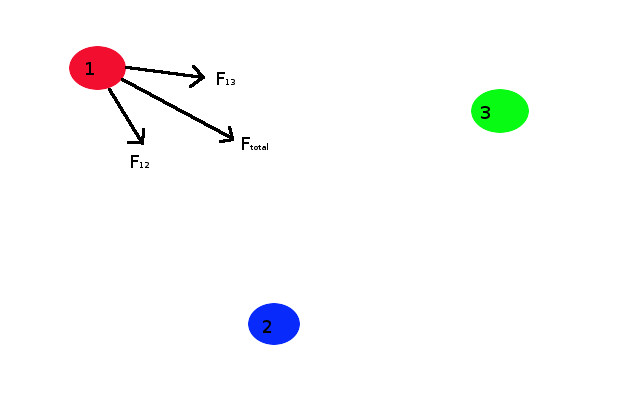
\includegraphics[scale=0.5]{vector}}

 This total force is given by the sum of all other forces acting on $P^x$ as crudely illustrated above.
Therefore $\vec{F}_{\sigma x}$ is given by 

\begin{equation}
\vec{F}_{\sigma x} = \sum_{n = 1, n \neq x}^{N} \vec{F}_{nx}
\end{equation}


\printbibliography
\end{document}
